\documentclass{article}

\usepackage{fancyhdr}
\usepackage{extramarks}
\usepackage{amsmath}
\usepackage{amsthm}
\usepackage{amsfonts}
\usepackage{tikz}
\usepackage[plain]{algorithm}
\usepackage{algpseudocode}
\usepackage[]{mcode}
\usepackage{graphicx}
\usepackage{epstopdf}
\usepackage{siunitx}
\usepackage{xfrac}

\usetikzlibrary{automata,positioning}

%
% Basic Document Settings
%

\topmargin=-0.45in
\evensidemargin=0in
\oddsidemargin=0in
\textwidth=6.5in
\textheight=9.0in
\headsep=0.25in

\linespread{1.1}

\pagestyle{fancy}
\lhead{\hmwkAuthorName}
\chead{\hmwkClass\ (\hmwkClassInstructor\ \hmwkClassTime): \hmwkTitle}
\rhead{\firstxmark}
\lfoot{\lastxmark}
\cfoot{\thepage}

\renewcommand\headrulewidth{0.4pt}
\renewcommand\footrulewidth{0.4pt}

\setlength\parindent{0pt}

%
% Create Problem Sections
%

\newcommand{\enterProblemHeader}[1]{
    \nobreak\extramarks{}{Problem \arabic{#1} continued on next page\ldots}\nobreak{}
    \nobreak\extramarks{Problem \arabic{#1} (continued)}{Problem \arabic{#1} continued on next page\ldots}\nobreak{}
}

\newcommand{\exitProblemHeader}[1]{
    \nobreak\extramarks{Problem \arabic{#1} (continued)}{Problem \arabic{#1} continued on next page\ldots}\nobreak{}
    \stepcounter{#1}
    \nobreak\extramarks{Problem \arabic{#1}}{}\nobreak{}
}

\setcounter{secnumdepth}{0}
\newcounter{partCounter}
\newcounter{homeworkProblemCounter}
\setcounter{homeworkProblemCounter}{1}
\nobreak\extramarks{Problem \arabic{homeworkProblemCounter}}{}\nobreak{}

%
% Homework Problem Environment
%
% This environment takes an optional argument. When given, it will adjust the
% problem counter. This is useful for when the problems given for your
% assignment aren't sequential. See the last 3 problems of this template for an
% example.
%
\newenvironment{homeworkProblem}[1][-1]{
    \ifnum#1>0
        \setcounter{homeworkProblemCounter}{#1}
    \fi
    \section{Problem \arabic{homeworkProblemCounter}}
    \setcounter{partCounter}{1}
    \enterProblemHeader{homeworkProblemCounter}
}{
    \exitProblemHeader{homeworkProblemCounter}
}

%
% Homework Details
%   - Title
%   - Due date
%   - Class
%   - Section/Time
%   - Instructor
%   - Author
%

\newcommand{\hmwkTitle}{Tutorial\ 6}
\newcommand{\hmwkDueDate}{May 21, 2017}
\newcommand{\hmwkClass}{Digital Signal Processing}
\newcommand{\hmwkClassTime}{}
\newcommand{\hmwkClassInstructor}{Friso DeBoer}
\newcommand{\hmwkAuthorName}{S.Reynolds (262538)}

%
% Title Page
%

\title{
    \vspace{2in}
    \textmd{\textbf{\hmwkClass:\ \hmwkTitle}}\\
    \normalsize\vspace{0.1in}\small{Due\ on\ \hmwkDueDate\ at 3:00pm}\\
    \vspace{0.1in}\large{\textit{\hmwkClassInstructor\ \hmwkClassTime}}
    \vspace{3in}
}

\author{\textbf{\hmwkAuthorName}}
\date{}

\renewcommand{\part}[1]{\textbf{\large Part \Alph{partCounter}}\stepcounter{partCounter}\\}

%
% Various Helper Commands
%

% Useful for algorithms
\newcommand{\alg}[1]{\textsc{\bfseries \footnotesize #1}}

% For derivatives
\newcommand{\deriv}[1]{\frac{\mathrm{d}}{\mathrm{d}x} (#1)}

% For partial derivatives
\newcommand{\pderiv}[2]{\frac{\partial}{\partial #1} (#2)}

% Integral dx
\newcommand{\dx}{\mathrm{d}x}

% Alias for the Solution section header
\newcommand{\solution}{\textbf{\large Solution}}

% Probability commands: Expectation, Variance, Covariance, Bias
\newcommand{\E}{\mathrm{E}}
\newcommand{\Var}{\mathrm{Var}}
\newcommand{\Cov}{\mathrm{Cov}}
\newcommand{\Bias}{\mathrm{Bias}}

\graphicspath{{../Images/}}

\begin{document}

\maketitle

\pagebreak

\section{Linear Interpolation}

\subsection{Part A \& Part B}

The warm up exercise provided code which took a 1D signal and provided a zoom on the signal, using a triangular filter to interpolate values. The code can be seen below:
\begin{lstlisting}
	% Clear any sotred variables, clear the workspace, and close any figures
	clear; clc; close all;
	
	xss = zeros(1,19);
	samp = [1 3 -2 4 2 -1 -3];
	xss(1:3:19) = samp;
	
	coeff = [1/3 2/3 1 2/3 1/3];
	output = firfilt(xss,coeff);
	
	subplot(2,1,1)
	stem(xss)
	xlabel('time')
	title('Original signal padded with zeros')
	axis([0 25 -4 4])
	
	subplot(2,1,2)
	stem(output)
	xlabel('time')
	title('Interpolated signal')
	axis([0 25 -4 4])
\end{lstlisting}

The plots of the original signal and the interpolated signal can be seen in Figure 1. We note that the lower plot has the zero values changed to values that provide a transition to non-zero values. Further, we see a shift in the filtered signal to the right by 2 time units.

\begin{figure}[H]
	\centering
	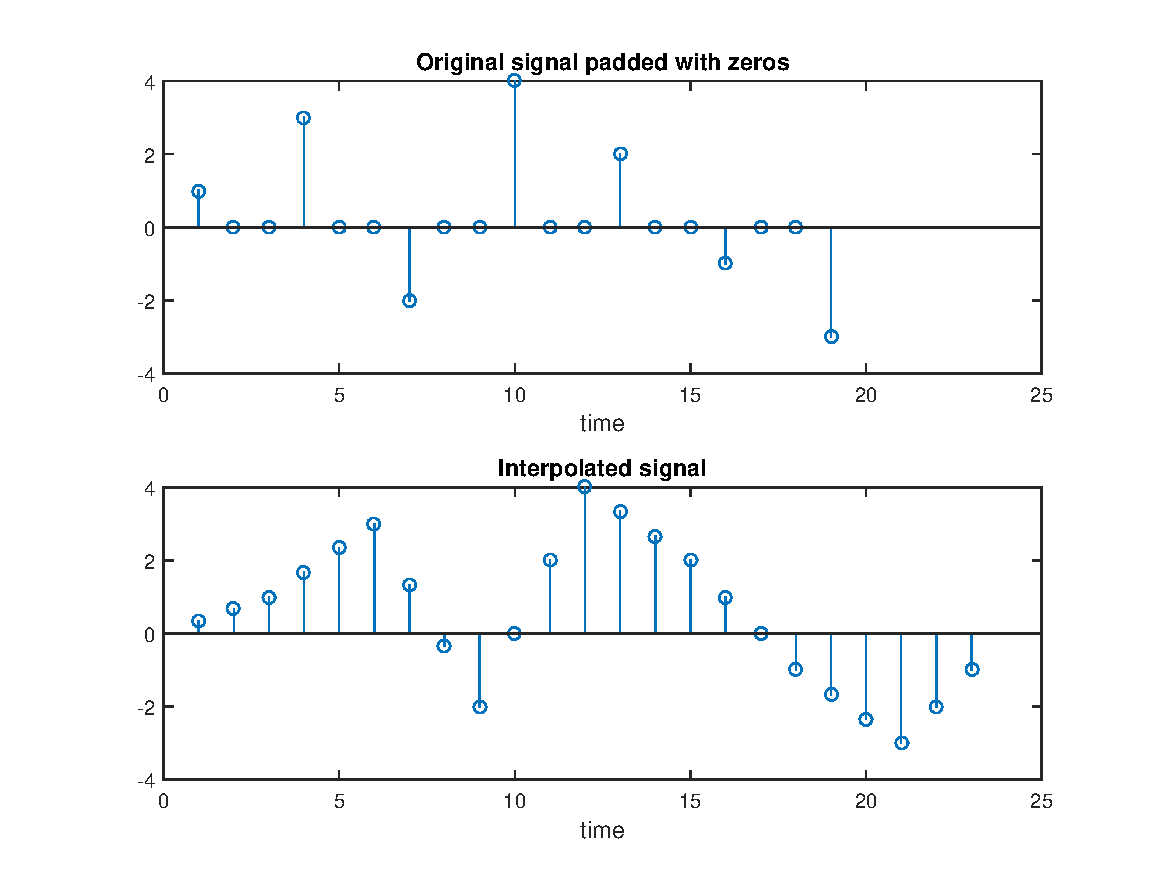
\includegraphics[scale=0.5]{fig1.eps}
	\caption{The top plot shows the original signal padded with zero values between actual data points. The lower plot shows the filtered signal which has values interpolated between the actual data values. Further, we note that the signal is delayed by 2 time units.}
\end{figure}

\subsection{Part C}

The difference equation for the interpolation filter used above, can be written simply by considering the $b_k$ coefficients. The difference equation is as follows:
\begin{align*}
	y[n] = \sfrac{1}{3} \cdot x[n] + \sfrac{1}{3} \cdot x[n-1] + x[n-2] + \sfrac{2}{3} \cdot x[n-3] + \sfrac{1}{3} \cdot x[n-4]
\end{align*}

Suppose the input signal to the interpolation filter was as follows:
\begin{align*}
	x[n] = \delta [n] + 0.5 \cdot \delta [n - 3]
\end{align*}

The output from the filter would be as follows:
\begin{align*}
	y[n] =& \quad \sfrac{1}{3} \cdot \delta [n] + \sfrac{1}{6} \cdot \delta [n-3] \\
	& \quad + \sfrac{2}{3} \cdot \delta [n-1] + \sfrac{2}{6} \cdot \delta [n-4] \\
	& \quad + \delta [n-2] + \sfrac{1}{2} \cdot \delta [n-5] \\
	& \quad + \sfrac{2}{3} \cdot \delta [n-3] + \sfrac{2}{6} \cdot \delta [n-6] \\
	& \quad + \sfrac{1}{3} \cdot \delta [n-4] + \sfrac{1}{6} \cdot \delta [n-7]
\end{align*}

\section{Sampling of Images}

\subsection{Part A}
Images that are stored on a computer are sampled images, which means that there are a discrete number of pixels stored in an $M \times N$ array. The sampling rate of the image was chose at the time the photograph is taken, however, the sampling rate can be changed by discarding pixel elements in a systematic way. The code shown below is the implementation of one such strategy, whereby every fourth pixel is discarded and replaced by a zero value. The code doesn't change the size of the image, rather it create a zero matrix of the same size as the original image, and then populates every fourth entry across the zero matrix by a one. Finally, to obtain the image at the lower sampling rate, the $M \times N$ matrix with zeros and ones is multiplied by the initial matrix in a piecewise fashion to achieve the result.

\begin{lstlisting}
	function  yy = imsample(xx, P)
	%IMSAMPLE    Function for sub-sampling an image
	%  usage:  yy = imsample(xx,P)
	%    xx = input image to be sampled
	%     P = sub-sampling period (a small integer like 2, 3, etc.)
	%    yy = output image
	%
	[M,N] = size(xx);
	S = zeros(M,N);
	S(1:P:M,1:P:N) = ones(length(1:P:M), length(1:P:N));
	yy = xx .* S;
\end{lstlisting}


\subsection{Part B}
The \verb|imsample| function was employed using the baboon image as part of the MATLAB package - the original image and the image with the lowered sampling rate can be seen in Figures 2 and 3, respectively. The MATLAB script used to implement the sampling at the lower rate can be seen in Appendix A.

\begin{figure}[H]
	\hspace{1cm}
	\begin{minipage}{0.5\linewidth}
		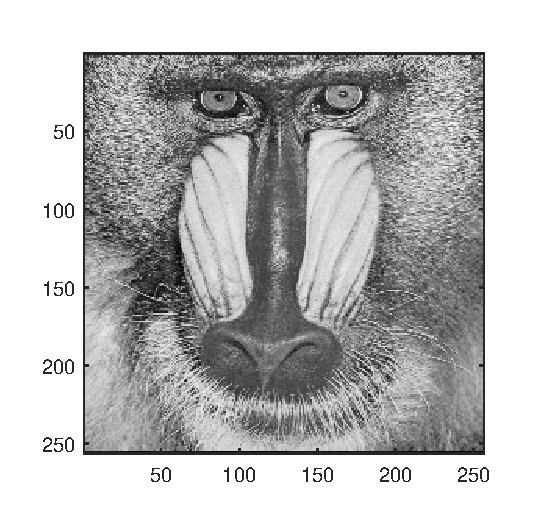
\includegraphics[scale=0.8]{fig2}
		\caption{Original image of the Baboon}
	\end{minipage}
	\begin{minipage}{0.5\linewidth}
		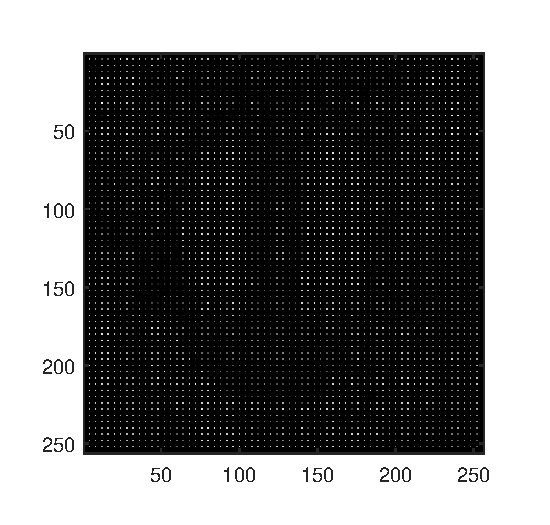
\includegraphics[scale=0.8]{fig3}
		\caption{Baboon image at a lower sampling rate}
	\end{minipage}
\end{figure}

\subsection{Part C}
Down sampling occurs when samples are thrown away and the image is resized. A drawback of employing this method is that aliasing may occur. The script in Appendix A demonstrates this effect.

\begin{figure}[H]
	\centering
	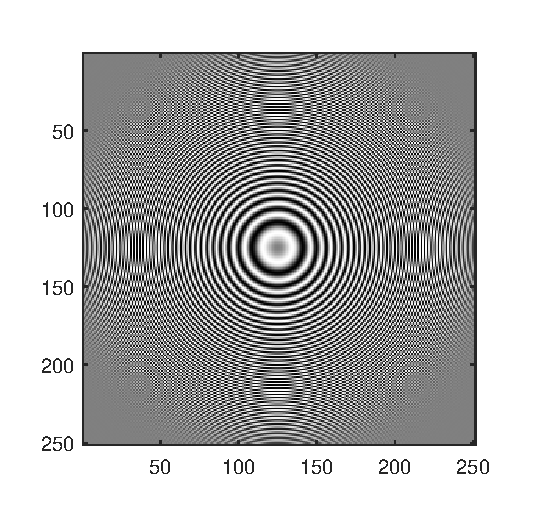
\includegraphics[scale=1.2]{fig5}
	\caption{A downsampled image of a zone plate. The aliasing effect shown in the image is the repetition of the central image throughout the remainder of the image.}
\end{figure}

\begin{figure}[H]
	\hspace{-2cm}
	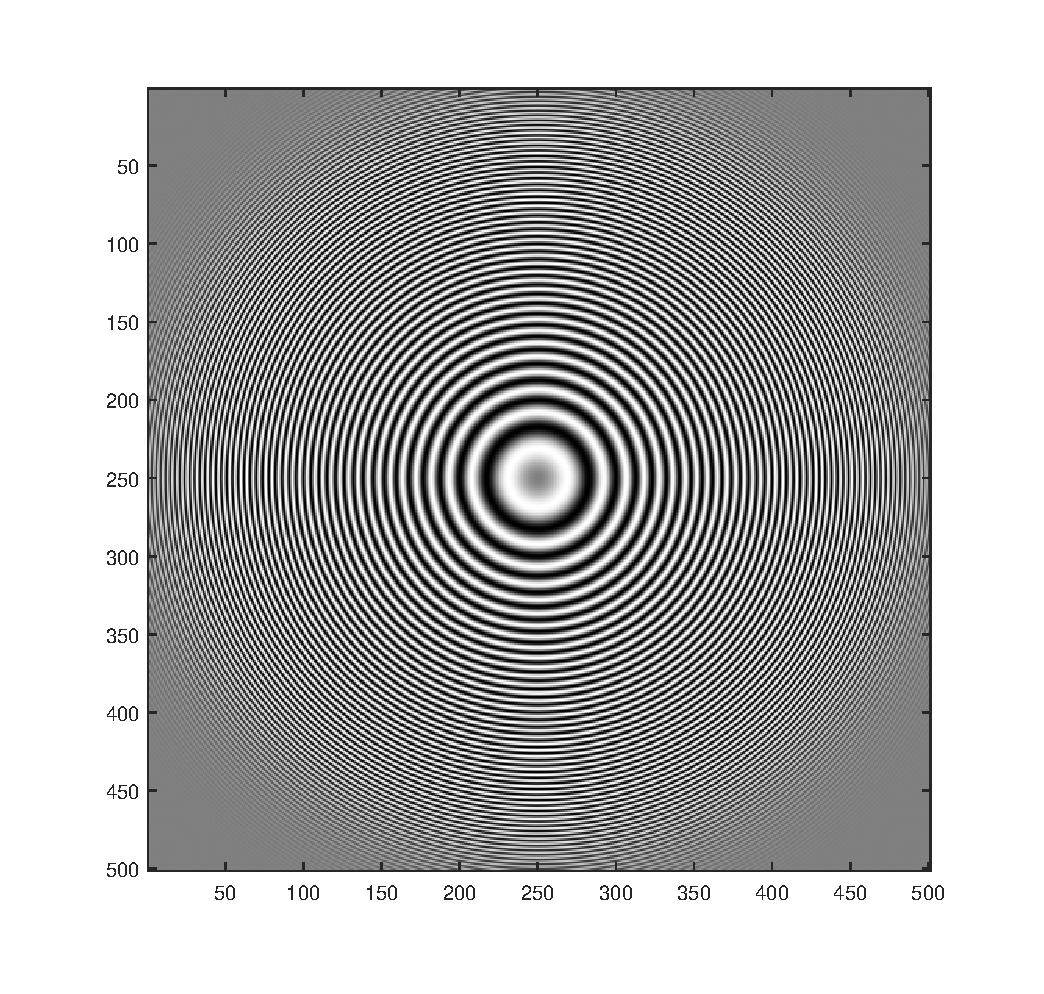
\includegraphics[scale=1.2]{fig4}
	\caption{The original zone plate image.}
\end{figure}

The zone plate is an image in which there are higher frequencies which are integer multiples of lower frequencies present in the image. The aliasing effect can be seen in Figure 4, and the original zone plate image can be seen over the page in Figure 5. Visually, the aliasing effect in static images sees appears as repetition of a central element of the image. In this instance we see the central pattern repeated throughout the image. The reason for the aliasing effect taking place is due to the sampling rate of the image being lowered below the recommended Nyquist sampling rate, which is 2 times the highest frequency present in the image.\\

The lenna image was also down sampled in the script shown in Appendix A. The original image can be seen in Figure 6 and the down sampled image can be seen in Figure 7. We note that the down sampled Lenna image has a higher level of distortion in the form of pixelation. Although there may be some aliasing in the down sampled Lenna image, it is not visually apparent. This is due to the reduced number of higher frequencies in the image which are multiples of lower frequencies.

\begin{figure}[H]
	\begin{minipage}[t]{0.5\linewidth}
		\centering
		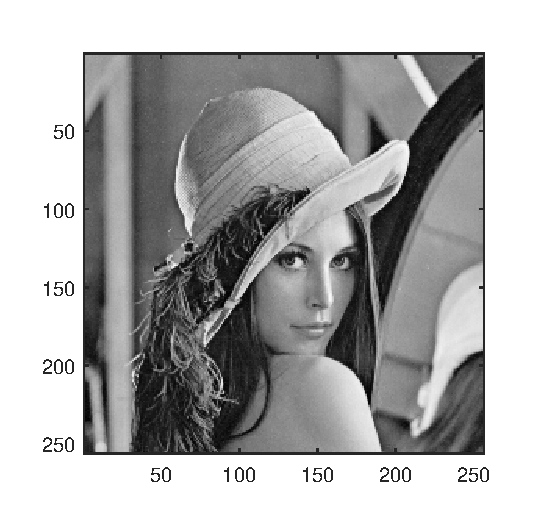
\includegraphics[scale=0.5]{fig6}
		\caption{Original Lenna image}
	\end{minipage}
	\begin{minipage}[t]{0.5\linewidth}
		\centering
		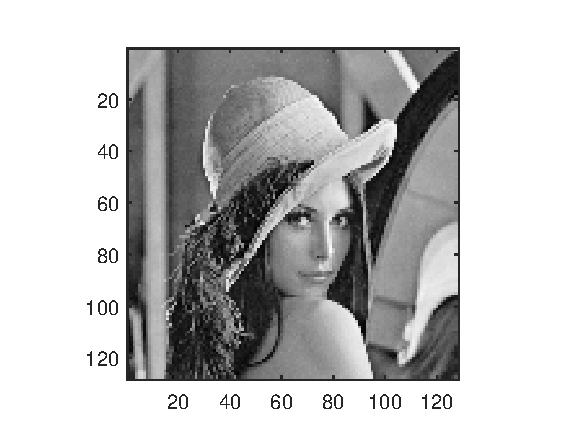
\includegraphics[scale=0.6]{fig7}
		\caption{Down sampled Lenna image}
	\end{minipage}
\end{figure}

\section{Reconstruction of Images}

\subsection{Part A}
A tools image, which is part of the MATLAB package, was imported and re-sampled at a lower sampling rate using the \verb|imsample| function - the result can be seen in Figure 8. A zero order hold image reconstruction was undertaken on the rows of the re-sampled image, which resulted in the partial reconstruction of the image, which can be seen in Figure 9. The MATLAB implementation of these operations can be seen in Appendix B.

\begin{figure}[H]
	\begin{minipage}{0.5\linewidth}
		\centering
		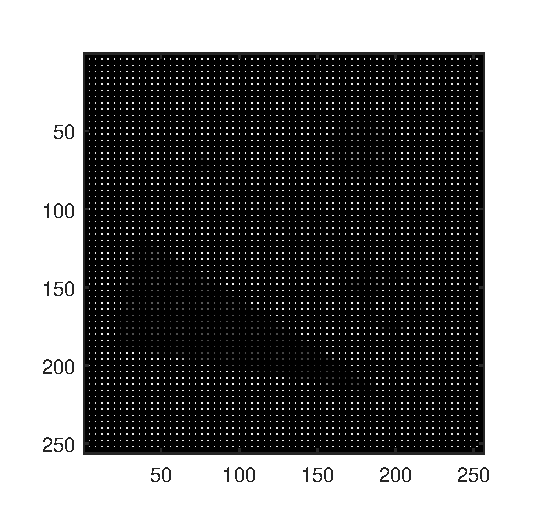
\includegraphics[scale=0.8]{fig8}
		\caption{text}
	\end{minipage}
	\begin{minipage}{0.5\linewidth}
		\centering
		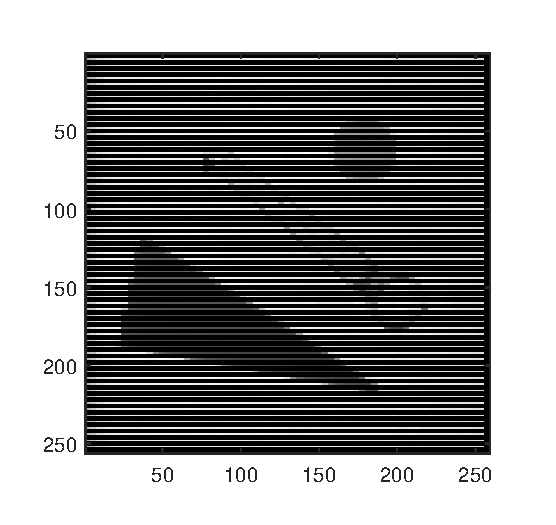
\includegraphics[scale=0.8]{fig9}
		\caption{text}
	\end{minipage}
\end{figure}

\subsection{Part B}
After the row interpolation, the script in Appendix B passes the filter over the columns of the lower rate tools image. The results can be seen in Figure 10. The Figure shows a successful reconstruction of the image using zero order hold interpolation filter, however, there is some loss of quality in comparison with the original image.  
\begin{figure}[H]
	\begin{minipage}{0.5\linewidth}
		\centering
		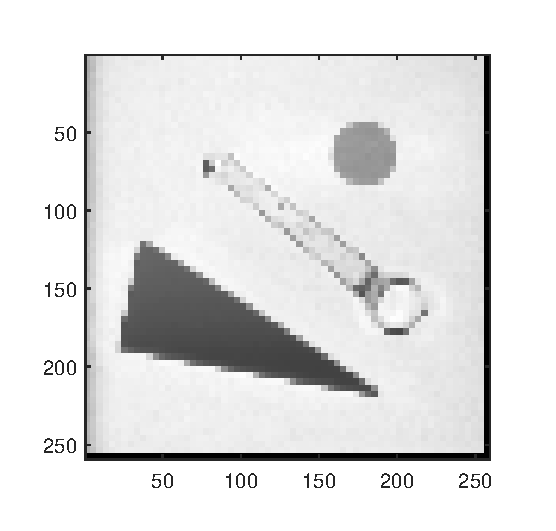
\includegraphics[scale=0.8]{fig10}
		\caption{Image reconstructed using a zero order hold FIR interpolation filter}
	\end{minipage}
\hspace{0.5cm}
	\begin{minipage}{0.5\linewidth}
		\centering
		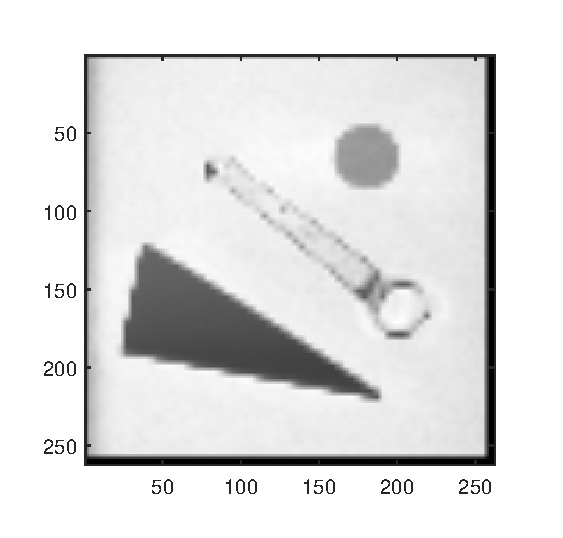
\includegraphics[scale=0.8]{fig11}
		\caption{Image reconstructed using a triangular FIR interpolation filter}
	\end{minipage}
\end{figure}

\subsection{Part C}
Linear interpolation uses a triangular filter on the rows and columns of the image. An FIR filter of order $M=6$ was used to filter the image. The $b_k$ parameters for the image are as follows:
\begin{align*}
	\{b_k\} = \{\sfrac{1}{4}, \quad \sfrac{2}{4}, \quad \sfrac{3}{4}, \quad 1, \quad \sfrac{3}{4}, \quad \sfrac{2}{4}, \quad \sfrac{1}{4}\}
\end{align*}

\subsection{Part D}
Linear interpolation was carried out using the triangular FIR filter, as seen in Appendix B. Figure 11 shows the resulting filtered image. There is a noticeable improvement in the quality of the reconstructed image using the triangular filter. In particular, there is less pixelation around the edges of objects in the image.

\newpage

\subsection{Part E}
Figure 12 shows the frequency response plot for the triangular FIR filter over the domain $-\pi \leq \hat{\omega} \leq \pi $.

\begin{figure}[H]
	\begin{minipage}[t]{0.48\linewidth}
		\centering
		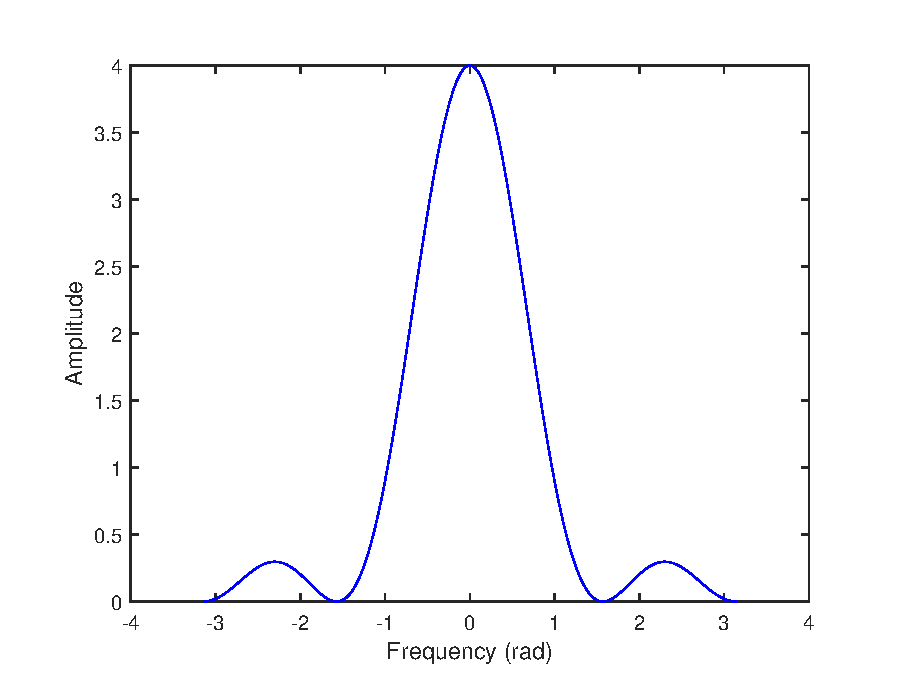
\includegraphics[scale=0.6]{fig12}
		\caption{The plot shows the magnitude of the frequency response for the triangular FIR filter of order $M=6$.}
	\end{minipage}
	\hspace{0.5cm}
	\begin{minipage}[t]{0.48\linewidth}
		\centering
		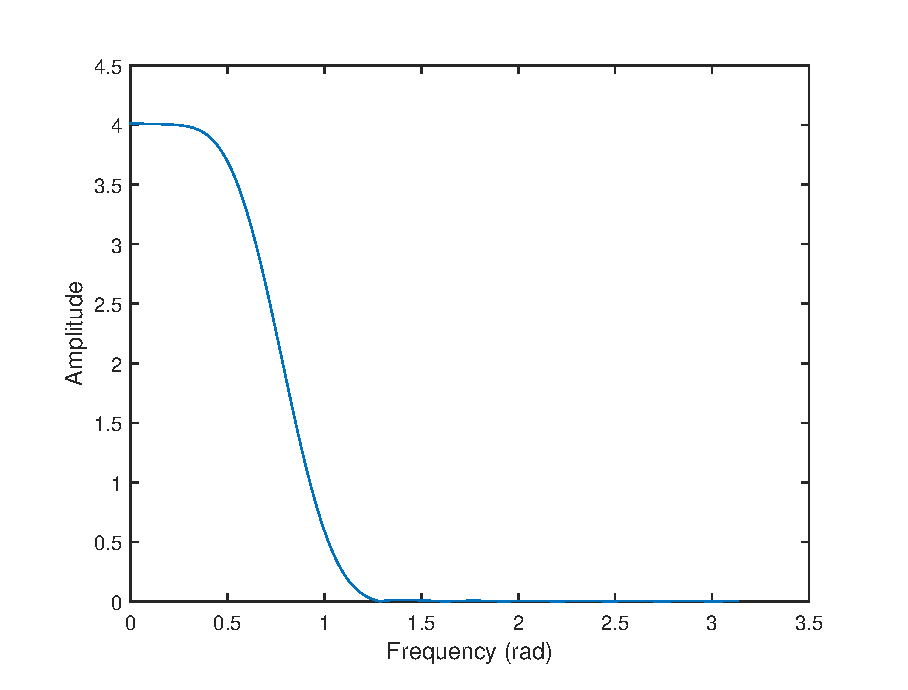
\includegraphics[scale=0.6]{fig14}
		\caption{The plot shows the magnitude of the frequency response for the 23-point FIR filter.}
	\end{minipage}
\end{figure}

\subsection{Part F}
A 23-point FIR lowpass filter was created using the following for the filter coefficients, $b_k$:
\begin{align}
	b_k = \frac{\sin (\sfrac{\pi (k-11)}{4})}{\sfrac{\pi(k-11)}{4}} \cdot \omega_k \quad k = 0,1,2,...,22
\end{align}

We note that $\omega_k$ is given by:
\begin{align}
	\omega_k = 0.54 - 0.46 \cdot \cos \bigg(\frac{2 \pi k}{22} \bigg) \quad k = 0,1,2,...,22
\end{align}

We note that at the instance $k = 11$, the filter coefficient $b_{11}$ is seemingly undefined. To show that this isn't the case, we consider the following limit of equation (1):
\begin{align*}
	\lim_{k \rightarrow 11} b_k 	&= \lim_{k \rightarrow 11} \frac{\sin (\sfrac{\pi (k-11)}{4})}{\sfrac{\pi(k-11)}{4}} \cdot \omega_k\\
									&= \bigg(\lim_{k \rightarrow 11} \frac{\sin (\sfrac{\pi (k-11)}{4})}{\sfrac{\pi(k-11)}{4}} \bigg) \cdot \bigg(\lim_{k \rightarrow 11} \omega_k \bigg)
\end{align*}

Letting $\xi = k-11$, we get:
\begin{align*}
	\lim_{k \rightarrow 11} b_k &= \bigg(\lim_{\xi \rightarrow 0} \frac{\sin (\xi)}{\xi} \bigg) \cdot \bigg(\lim_{k \rightarrow 11} \omega_k \bigg)\\
								&= 1 \cdot 1\\
								&= 1
\end{align*}

Figure 13 shows the frequency response of the 23-point low pass filter. We note that the filter lets more of the low frequencies through and has a sharper drop off - similar to an ideal LPF. The filter was used to reconstruct the image with the lower sampling rate. This was implemented in the MATLAB code shown in Appendix B, and Figure 14 shows the results of the filtering process.

\begin{figure}
	\centering
	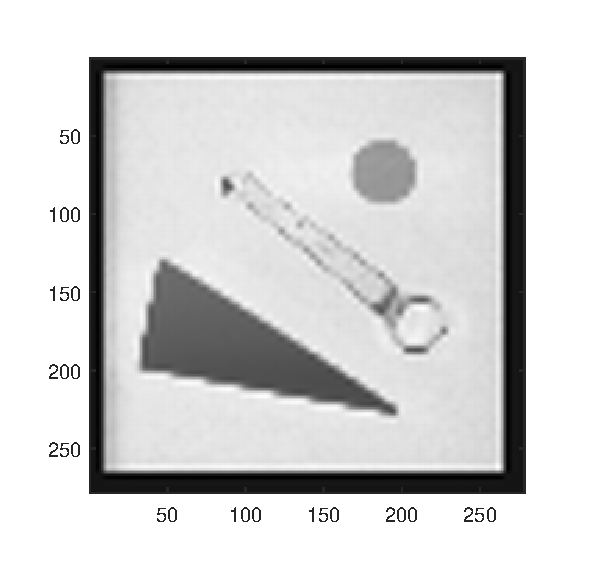
\includegraphics[scale=0.8]{fig13}
	\caption{The reconstructed image using the 23-point LPF shown in equations (1) and (2).}
\end{figure}

\section{Zooming for an Image}

\subsection{Part A}
A small 50$\times$50 section of the Lenna image was taken - her eye. By repeating the pixel elements 4 times in each direction, we can zoom in on the image. This was implemented in a script in MATLAB which is listed in Appendix C - the resulting image from this zooming technique can be seen in Figure 15. We note that the image has suffered from some pixelation in te zooming process.
\begin{figure}[H]
	\centering
	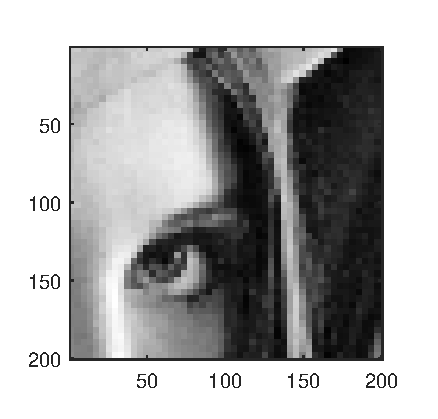
\includegraphics[scale=1]{fig15}
	\caption{A zoomed in image of the }
\end{figure} 

\subsection{Part B}
Another way to produce a larger image is by inserting zeros into the image around pixel values and then using an interpolation filter to smoother out the values. The zero padding function called \verb|zero_insert| is as follows:
\begin{lstlisting}
function yy = zero_insert(xx)
	[M,N] = size(xx);
	yy = zeros(4*M,4*N);
	yy(4:4:4*M,4:4:4*N) = xx;
end
\end{lstlisting}

\subsection{Part C}
The image with the zeros inserted into it was filtered using the triangular interpolation FIR, and the low pass filter seen in the previous section. The results of image filtering can be seen in Figures 16 and 17, respectively.
\begin{figure}[H]
	\begin{minipage}[t][][b]{0.48\linewidth}
		\centering
		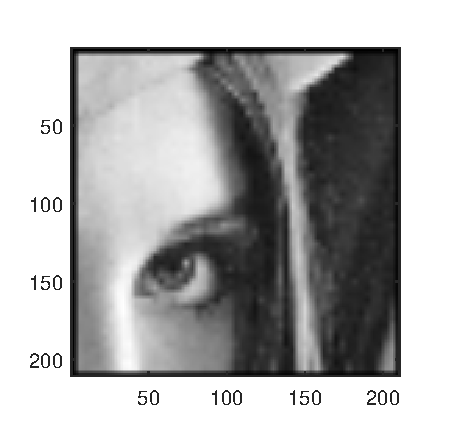
\includegraphics[scale=0.86]{fig16}
		\caption{Image filtered using the triangular filter developed in the previous section}
	\end{minipage}
\hspace{0.5cm}
	\begin{minipage}[t][][b]{0.48\linewidth}
		\centering
		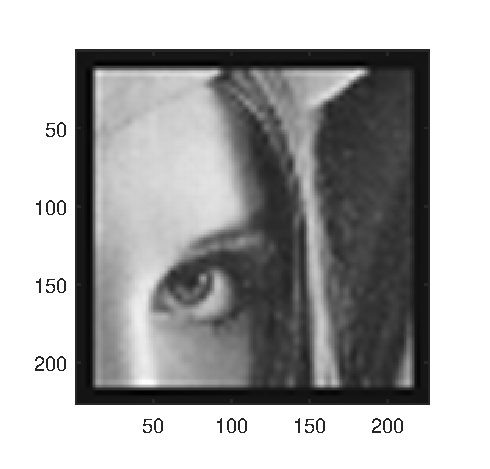
\includegraphics[scale=0.8]{fig17}
		\caption{Image filtered using the low pass filter developed in the previous section}
	\end{minipage}
\end{figure} 

The image using the low pass filter or the triangular interpolation have a similar effect on increasing the quality of the zoomed image, when compared to the pixel repetition method used in part A.

\newpage

\section{Appendix A}
\begin{lstlisting}
% Clear any existing variables, clear the workspace, and close figures
clear; clc; close all;

% Load the baboon image and employ downsampling
load baboon.mat
show_img(xx,1)
xs = imsample(xx,4); %-- Sample every fourth point in the image
show_img(xs,2)

% Load the zone plate image and downsample to observe aliasing
x1 = imzoneplate; %-- Create the zoneplate image
show_img(x1,3)
[M,N] = size(x1);
p = 2;
xp = x1(1:p:M,1:p:N); %-- Downsample the image
show_img(xp,4)

% Load the lenna image and downsample to observe the lack of
% aliasing
load lenna.mat
show_img(xx,5)
[M,N] = size(xx);
p = 2;
xp = xx(1:p:M,1:p:N); %-- Downsample the image
show_img(xp,6)
\end{lstlisting}

\newpage

\section{Appendix B}
\begin{lstlisting}
% Clear any stored variables, clear the workspace, and close all figures
clear; clc; close all;

% Load the images into the workspace
load tools.mat

% Downsample the image
xs = imsample(xx,4);

% Create a zero hold interpolation filter
bs = ones(1,4);

% Filter the downsized data
yhold = conv2(xs,bs);
hold_final = conv2(yhold,bs');

% Show all three images
show_img(xs,1) %-- original image
show_img(yhold,2) %-- horizontal filter
show_img(hold_final,3) %-- horizontal and vertical filter

% Linear interpolation filter
bk = [1/4 2/4 3/4 1 3/4 2/4 1/4];

% Filter the downsize data uing the linear filter
ylin = conv2(xs,bk); %-- filter rows
ylin = conv2(ylin,bk'); %-- filter columns
show_img(ylin,4)

% Determine the frequency response for the filter
[H,W] = freqz(bk);
figure(5)
plot(W,abs(H),'b')
hold on
plot(-W,abs(H),'b')
xlabel('Frequency (rad)')
ylabel('Amplitude')

% Lowpass sinc function filter
k = 0:22;
wk = 0.54 - 0.46*cos((2*pi*k)/(22));
bkk = ( (sin((k-11)*(pi/4)))./((k-11)*(pi/4)) ).*wk;
bkk(12) = 1;

% Filter the downsized image using the low pass mdoified
% sinc filter
xs_filt = conv2(xs,bkk); %-- filter rows
xs_filt = conv2(xs_filt,bkk'); %-- filter columns

show_img(xs_filt,6)

[H,W] = freqz(bkk);
figure(7)
plot(W,abs(H))
xlabel('Frequency (rad)')
ylabel('Amplitude')
\end{lstlisting}

\newpage

\section{Appendix C}
\begin{lstlisting}
% Clear variables, clear the workspace, and close all figures
clear; clc; close all;

load lenna.mat

% Selection of the area on which to zoom
xx_sub = xx(100:150,150:200);

% Method 1 - Zooming by repeating values
xx_new = zeros(200,200);
a = 1;
b = 1;

for i = 1:50
	a = ( (i-1)*4 + 1 ):( (i-1)*4 + 1 + 3 );
		for j = 1:50
			b = ( (j-1)*4 + 1 ):( (j-1)*4 + 1 + 3 );
			xx_new(a,b) = xx_sub(i,j);
		end
end

show_img(xx_new,1)

% Method 2 - Zooming by filtering with linear interpolator
yy = zero_insert(xx_sub); %-- create matrix to be filtered

bk = [1/4 2/4 3/4 1 3/4 2/4 1/4]; %-- linear interpolation filter
ylin = conv2(yy,bk); %-- filter rows
ylin = conv2(ylin,bk'); %-- filter columns
show_img(ylin,2)

% Method 3 - Zooming by filtering with sinc filter

% Sinc filter creation
k = 0:22;
wk = 0.54 - 0.46*cos((2*pi*k)/(22));
bkk = ( (sin((k-11)*(pi/4)))./((k-11)*(pi/4)) ).*wk;
bkk(12) = 1;

xs_filt = conv2(yy,bkk); %-- filter rows
xs_filt = conv2(xs_filt,bkk'); %-- filter columns
show_img(xs_filt,3)
\end{lstlisting}
\end{document}